\chapter{Progetto 2: Compressione di immagini tramite la DCT}

\section{Introduzione}
Per la realizzazione della compressione di immagini, è stato scelto di utilizzare
\href{https://julialang.org/}{\textbf{Julia}}, per i medesimi motivi del progetto
precedente.

In questo progetto è stata implementata l'equazione della discrete cosine transform $2$ (DCT2).
La sua implementazione è stata realizzata applicando sequenzialmente sulla matrice
la discrete cosine transform $1$ (DCT) prima per righe e poi
per colonne. In questo modo, è stata aumentata la riutilizzabilità del codice
e ridotto il rischio di introdurre errori.

In particolare per lo sviluppo sono state utilizzate le librerie:
\begin{itemize}
    \item \textbf{LinearAlgebra}
    \item \textbf{FileIO}: fornisce funzioni per la lettura e scrittura di file.
    \item \textbf{Images}: fornisce funzioni per la trattazione di immagini.
    \item \textbf{\href{https://github.com/JuliaMath/FFTW.jl}{FTTW}}: fornisce
          funzioni che implementano la FTT.
\end{itemize}

Tutte le librerie sono open source, più precisamente FTTW implementa un binding
con la libreria di C.

\section{DCT2 custom}
Per prima cosa è stata implementata DCT1,
la cui sua formula è stata riportata nell'equazione \ref{eq:dct}.

\begin{equation}
    X_k = \begin{cases}
        \sqrt{\frac{1}{N}}\cdot \sum_{n=0}^{N-1} x_n \cos\left[\frac{\pi}{N}\left(n + \frac{1}{2}\right) n \right] & k=1     \\
        \sqrt{\frac{2}{N}}\cdot\sum _{n=0}^{N-1}x_{n}\cos \left[\frac{\pi}{N}\left(n+\frac{1}{2}\right)n\right]    & k \ne 1
    \end{cases}
    \label{eq:dct}
\end{equation}

Per l'implementazione, si è pensato di utilizzare un approccio basato su operazioni
tra vettori e matrici, più precisamente si pre-calcola la matrice
della base dei coseni (per righe) prima di effettuare il calcolo dei coefficienti.
Successivamente si effettua un prodotto matrice-vettore per ottenere il vettore
dei coefficienti, infine si normalizza il vettore dei coefficienti.

Dato un generico vettore $X_k$, per applicare la DCT si effettua:
\begin{equation*}
    dct(X_k) = norm(B_{\cos}\cdot X_k )
\end{equation*}

dove $\cdot$ rappresenta il prodotto matrice-vettore, $B_{\cos}$
è la base dei coseni creata per riga e $X_k$ è il vettore colonna iniziale.
I coefficienti così ottenuti vengono normalizzati nel seguente modo:
\begin{itemize}
    \item Il primo coefficiente viene moltiplicato per $\sqrt{\frac{1}{N}}$
    \item I restanti vengono moltiplicati per $\sqrt{\frac{2}{N}}$
\end{itemize}

L'implementazione della DCT2 si articola nel seguente modo:
\begin{itemize}
    \item si genera la base dei coseni per riga
    \item si applica inplace la DCT1 per righe
    \item si applica inplace la DCT1 per colonne
\end{itemize}

Utilizzando questa strategia si riesce ad ottenere dei tempi di esecuzione
comparabili alla DCT2 implementata dalla libreria usando la FFT.

Il codice della DCT è all'interno del file \textbf{Dct2.jl}, mentre il codice dei
test della dct e il codice per generare il grafico di complessità è nella cartella
\textbf{test\_dct.jl}.

\subsection{Studio di complessità}

La complessità della DCT2 custom viene analizzata per passi nei seguenti punti:
\begin{itemize}
    \item \textbf{generazione della base dei coseni}: questa operazione richiede
          un numero costante di operazioni tra scalari e un calcolo del coseno per ogni
          entry della matrice. Avremo quindi un totale $\mathcal{O}(N^2)$ per generare
          la matrice, quando $N\times N$ è la dimensione della matrice.
    \item \textbf{applicazione della DCT1 su un vettore}: richiede di effettuare
          un prodotto matrice-vettore e successivamente di normalizzare i coefficienti.
          Il prodotto matrice-vettore ha una complessità asintotica di
          $\mathcal{O}(N^2)$, dove $N$ è la dimensione del vettore. Mentre per
          normalizzare i coefficienti si richiede una scansione
          lineare del vettore che richiede $\mathcal{O}(N)$, dove $N$ è la dimensione
          del vettore. Quindi complessivamente si ha una complessità di $\mathcal{O}(N^2 + N) = \mathcal{O}(N^2)$.
    \item \textbf{applicazione della DCT2 sull'intera matrice}: l'applicazione della DCT2
          sull'intera matrice richiede di eseguire una DCT1 per ogni riga e poi per ogni
          colonna. All'atto pratico, non si rigenera ogni volta la matrice dei coseni,
          bensì inizialmente la si pre-calcola ($\mathcal{O}(N^2)$), successivamente si
          esegue la DCT1 per righe che richiede $\mathcal{O}(N \cdot N^2)$ ($N$ righe
          per $N^2$ la moltiplicazione riga-matrice) e successivamente si applica la
          DCT1 per colonne che richiede $\mathcal{O}(N \cdot N^2)$ ($N$ colonne
          per $N^2$ la moltiplicazione riga-matrice). Complessivamente si ottiene
          un $\mathcal{O}(N^3)$ a livello asintotico.
\end{itemize}

L'implementazione custom della DCT2 è stata confrontata anche con quella ottimizzata
dalla libreria usando la FFT e nell'immagine \ref{fig:analisi_complex} si
può vedere il confronto.

Per generare il grafico è stata utilizzata la libreria standard \textbf{Plot} ed
è stata utilizzata la macro \textbf{@elapsed} per ottenere i tempi di esecuzione
delle funzioni.

Tutti i test sono stati realizzati su una macchina con:
\begin{itemize}
    \item Sistema Operativo: Windows $11$
    \item CPU: Ryzen $7$ $4800H$
    \item RAM: $16GB$
    \item Julia: versione 1.10.2
\end{itemize}

\newpage
\begin{figure}[!ht]
    \centering
    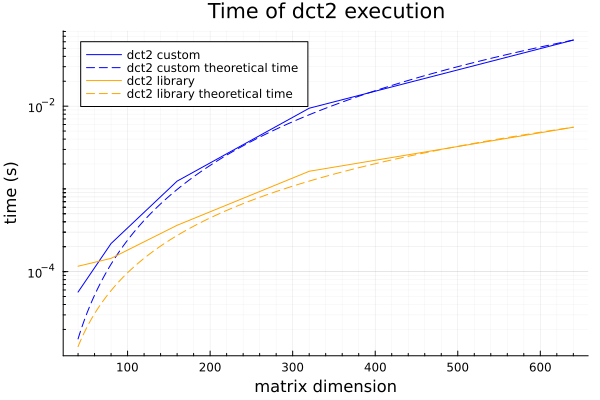
\includegraphics[width=0.5\textwidth]{Progetto_2/img/times_plot.png}
    \caption{Grafico dei tempi al variare della dimensione della matrice. Le linee
        continue rappresentano i dati empirici, le linee tratteggiate rappresentano
        l'andamento teorico dei metodi.}
    \label{fig:analisi_complex}
\end{figure}

Come si può notare dal grafico, l'andamento empirico segue quello teorico, ovvero
la DCT custom segue $\mathcal{O}(N^3)$, mentre la DCT della libreria segue $\mathcal{O}(N^2\log N)$.

In aggiunta, parlando dello spazio occupato, la DCT custom necessita di una matrice
$N \times N$ della base dei coseni e alloca un array di dimensione $N$ per salvare
i coefficienti, quindi si ottiene una complessità spaziale di $\mathcal{O}(N^2)$.

Si può ridurre la complessità spaziale effettuando tutte le operazioni inplace.

\section{Compressione}
Per facilitare l'uso del software che comprime l'immagine in scala di grigi, si
è pensato di sviluppare un'interfaccia mediante l'utilizzo di un framework open
source chiamato \href{https://github.com/plotly/dash}{Dash}. Il quale è un binding
in Julia della sua controparte in Python, generalmente utilizzato per data
visualizzation.

\subsection{Implementazione dell'interfaccia}
L'interfaccia consiste in una pagina web che chiede in input l'immagine da comprimere
e i parametri di compressione ($f$ e $d$), in output restituisce l'immagine compressa.

Nell'interfaccia vengono mostrate entrambe le immagini, sia quella di input sia quella
compressa, in modo da confrontare la qualità delle immagini.

Il sorgente dell'interfaccia è contenuto all'interno del file \textbf{gui.jl}.

Una volta che il server web è in esecuzione, per accedere all'interfaccia basta
digitare sul browser il seguente link: \href{http://localhost:8050}{http://localhost:8050}.

\subsection{Implementazione della compressione}
Dopo l'implementazione della GUI che si occupa di prendere in input l'immagine e
i due parametri, è stato sviluppato l'algoritmo di compressione dell'immagine.
L'algoritmo è all'interno del file \textbf{Dct2.jl} sotto la funzione \textbf{ApplyDct2OnImage}.

L'implementazione della compressione si articola nei seguenti passi:
\begin{itemize}
    \item \textbf{ridimensionamento dell'immagine in input}: l'immagine è stata
          ridimensionata in modo tale da avere altezza e larghezza multiple del
          parametro $f$.
    \item \textbf{implementazione della compressione}: la compressione è stata
          implementata applicando sui sotto-quadrati $f\times f$ dell'immagine
          la DCT2 della libreria, successivamente sono state azzerate le entry
          $M_{k,l}$ tali che $k+l\ge d$, infine si applica IDCT2 della libreria e
          si normalizzano i valori.
    \item \textbf{visualizzazione output}: infine viene visualizzato l'output
          messo a confronto con l'input.
\end{itemize}

Nel dettaglio, la \textbf{ridimensionamento dell'immagine in input} elimina le ultime
righe e le ultime colonne dell'immagine in input in modo da avere le dimensioni
multiple di $f$.

Mentre, l'\textbf{implementazione della compressione} si articola nell'allocazione
di una matrice di appoggio $C\in \mathbb{R}^{f\times f}$ che viene inizializzata
con una sotto-matrice $f\times f$ dell'immagine che si vuole elaborare. Successivamente
si applica la DCT2 della libreria, si azzerano i coefficienti $C_{kl}$ tali che
$k+l\ge d$, in seguito si applica la IDCT2 della libreria, infine si arrotondano
all'intero più vicino i coefficienti e si riportano i valori superiori a $255$
e inferiori a $0$ rispettivamente ai valori $255$ e $0$. Infine, si copia la
sotto-matrice di appoggio nell'immagine. Questo passo viene ripetuto in tutta
l'immagine suddividendola in blocchi $f \times f$ disgiunti.

Nella figura \ref{fig:compress} è possibile vedere l'esecuzione dell'algoritmo di
compressione su un imagine in bianco e nero utilizzando diversi parametri.

\begin{figure}[!ht]
    \centering
    \begin{subfigure}[!ht]{0.45\textwidth}
        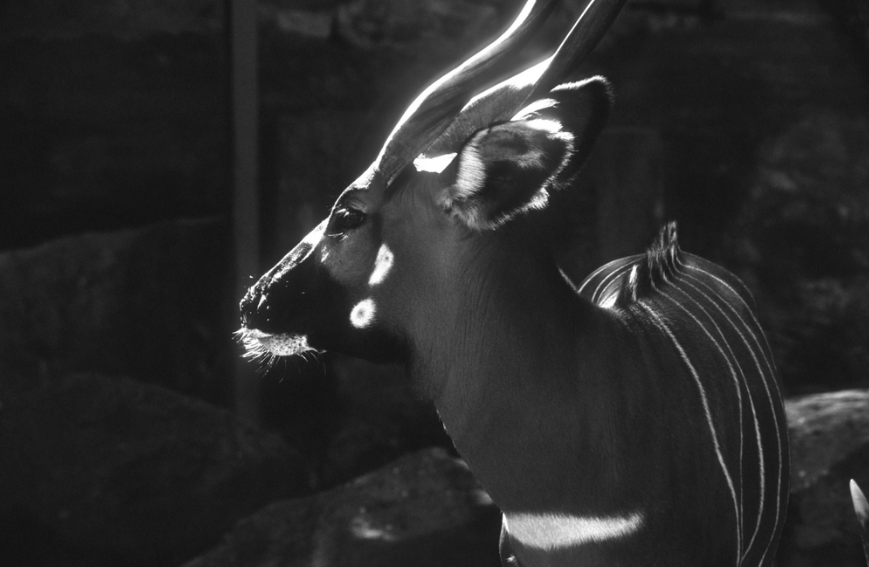
\includegraphics[width=\textwidth]{Progetto_2/img/gui.png}
        \caption{Immagine originale.}
    \end{subfigure}
    \begin{subfigure}[!ht]{0.45\textwidth}
        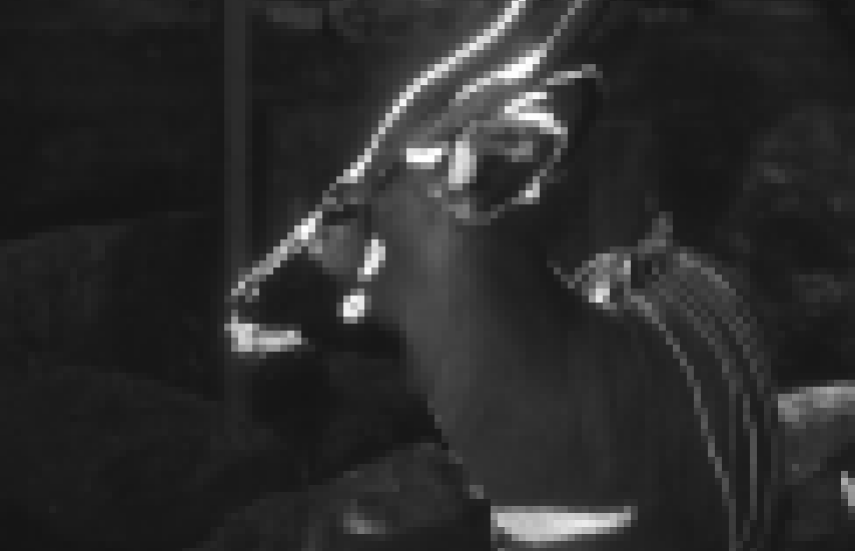
\includegraphics[width=\textwidth]{Progetto_2/img/gui_compressed1.png}
        \caption{Immagine compressa $f = 8$ e $d = 1$.}
    \end{subfigure}
    \begin{subfigure}[!ht]{0.45\textwidth}
        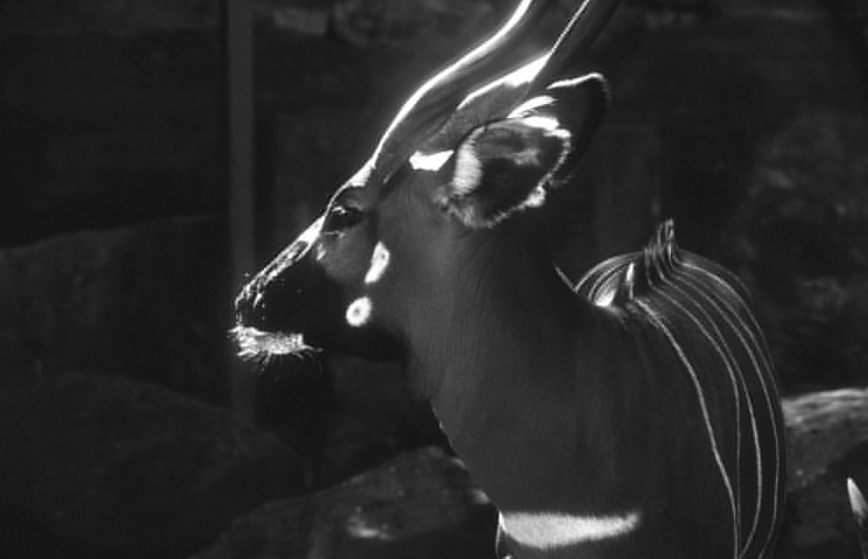
\includegraphics[width=\textwidth]{Progetto_2/img/gui_compressed.png}
        \caption{Immagine compressa $f = 8$ e $d = 4$.}
    \end{subfigure}
    \begin{subfigure}[!ht]{0.45\textwidth}
        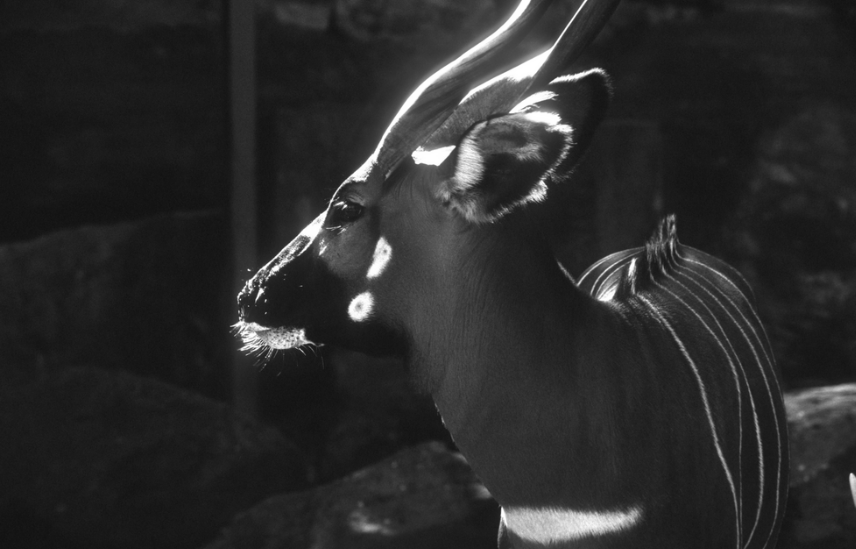
\includegraphics[width=\textwidth]{Progetto_2/img/gui_compressed14.png}
        \caption{Immagine compressa $f = 8$ e $d = 14$.}
    \end{subfigure}
    \caption{Esempi di esecuzione dell'algoritmo di compressione usando diversi 
    parametri}
    \label{fig:compress}
\end{figure}

Nelle figure si può notare che tenendo fissato il valore di $f$ la qualità dell'immagine 
peggiora al diminuire di $d$. Questo è un comportamento prevedibile dal momento 
che $d$ specifica quanti pixel preservare nelle sotto-matrici $f\times f$, perciò
più riduciamo e peggiore sarà la qualità dell'immagine con una presenza dei fenomeni 
di Gibbs.

Successivamente è stato rieseguito l'algoritmo di compressione sulla stessa immagine 
ma raddoppiando il valore di $f$ e mantenendo invariate le proporzioni di $d$ rispetto 
al caso precedente (vedi figure \ref{fig:compress2}). 

\begin{figure}[!ht]
    \centering
    \begin{subfigure}[!ht]{0.45\textwidth}
        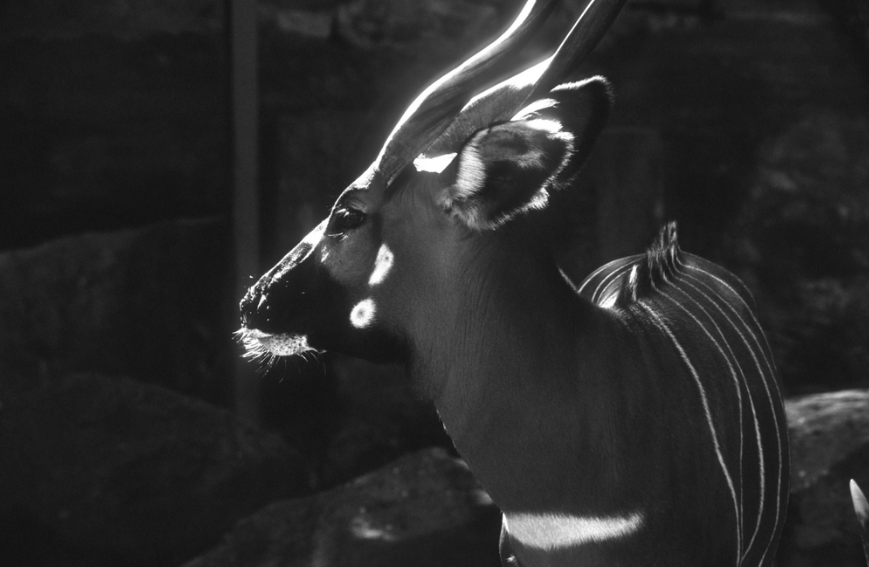
\includegraphics[width=\textwidth]{Progetto_2/img/gui.png}
        \caption{Immagine originale.}
    \end{subfigure}
    \begin{subfigure}[!ht]{0.45\textwidth}
        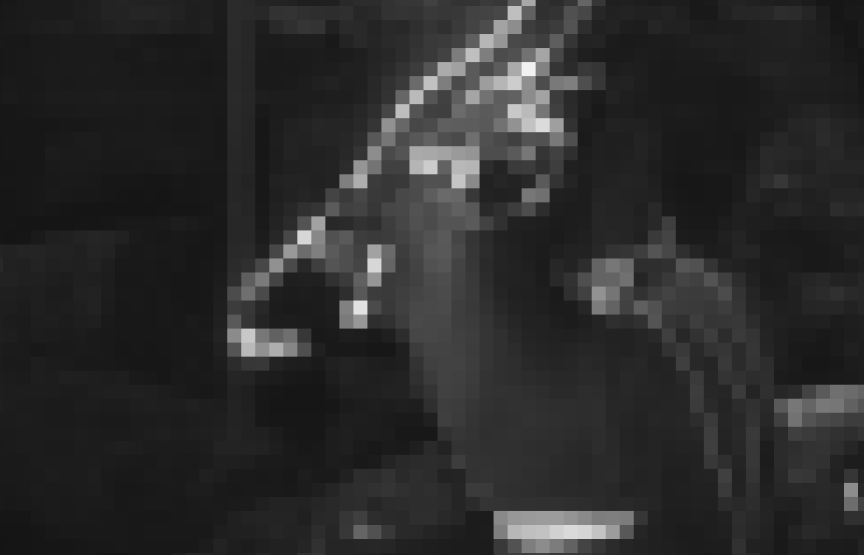
\includegraphics[width=\textwidth]{Progetto_2/img/f16d1.png}
        \caption{Immagine compressa $f = 16$ e $d = 1$.}
    \end{subfigure}
    \begin{subfigure}[!ht]{0.45\textwidth}
        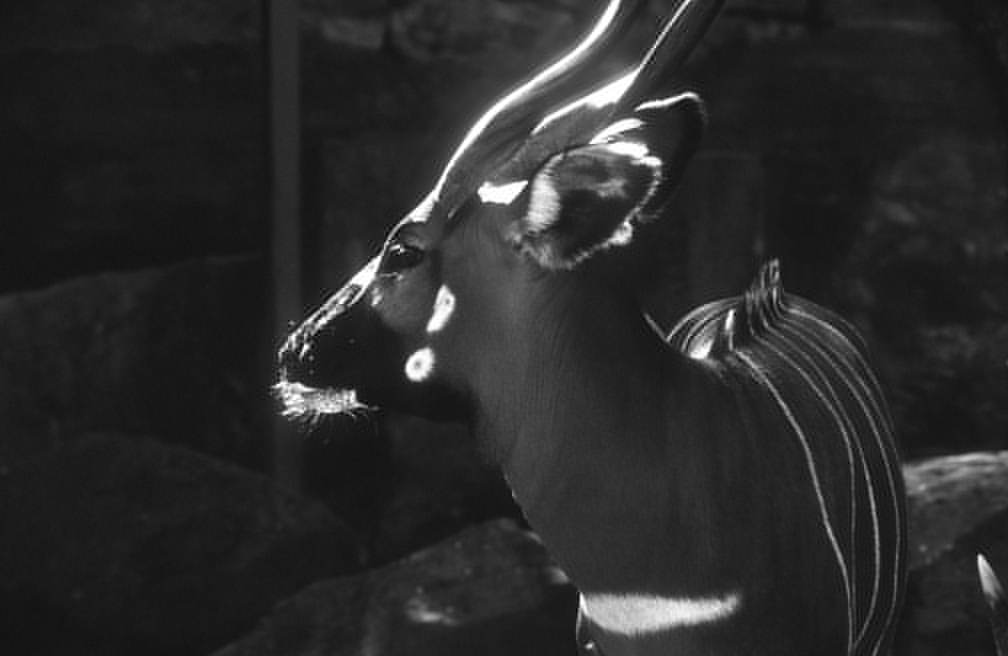
\includegraphics[width=\textwidth]{Progetto_2/img/f16d8.png}
        \caption{Immagine compressa $f = 16$ e $d = 8$.}
    \end{subfigure}
    \begin{subfigure}[!ht]{0.45\textwidth}
        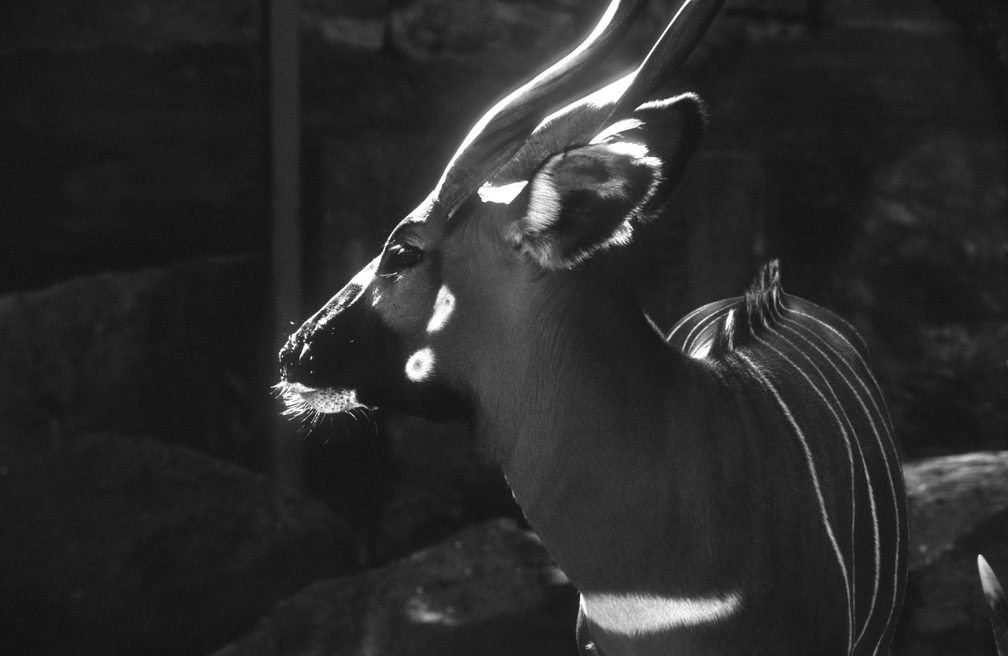
\includegraphics[width=\textwidth]{Progetto_2/img/f16d30.png}
        \caption{Immagine compressa $f = 16$ e $d = 30$.}
    \end{subfigure}
    \caption{Esempi di esecuzione dell'algoritmo di compressione usando diversi 
    parametri}
    \label{fig:compress2}
\end{figure}

In questo test si può notare come con la stessa proporzione di 
pixel preservati nelle sotto-matrici $f\times f$, si notano maggiormente la suddivisione 
dell'immagine in sotto matrici $f\times f$. Questo conferma le motivazioni 
teoriche nel mantenere il parametro $f$ basso per ridurre la fuoriuscita dei 
fenomeni di Gibbs.